\begin{figure}
    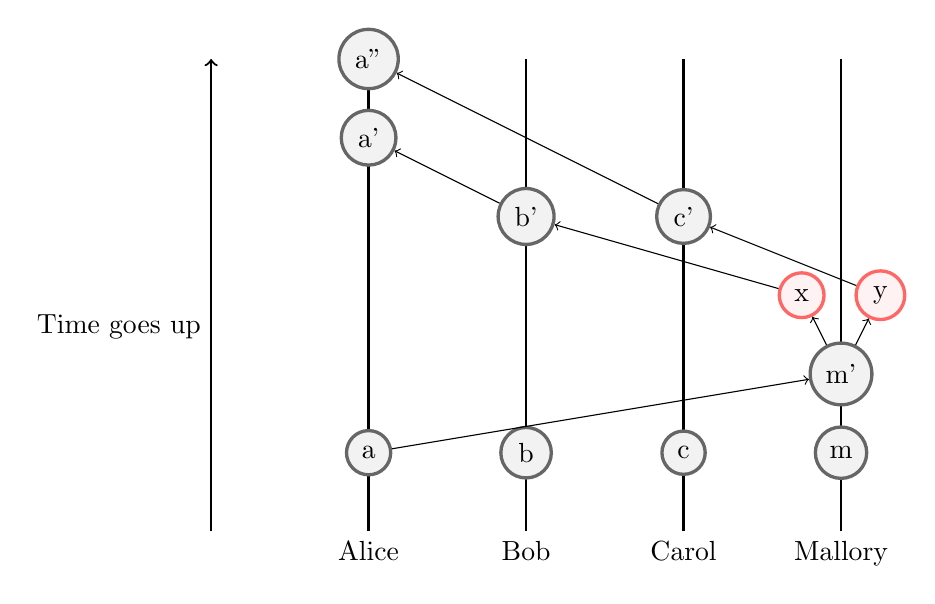
\begin{tikzpicture}[
        roundnode/.style={circle, draw=black!60, fill=black!5, very thick},
        rednode/.style={circle, draw=red!60, fill=red!5, very thick},
        ]
        \draw[thick,->] (0,0) -- (0,2.6) node[anchor=east] {Time goes up} -- (0,6);
        \draw[thick] (2,0) node[anchor=north] {Alice} -- (2,6);
        \draw[thick] (4,0) node[anchor=north] {Bob} -- (4,6);
        \draw[thick] (6,0) node[anchor=north] {Carol} -- (6,6);
        \draw[thick] (8,0) node[anchor=north] {Mallory} -- (8,6);
        
        % Nodes
        \node[roundnode] (a1) at (2,1) {a};
        \node[roundnode] (b1) at (4,1) {b};
        \node[roundnode] (c1) at (6,1) {c};
        
        \node[roundnode] (b4) at (4,4) {b'};
        \node[roundnode] (c4) at (6,4) {c'};

        % Nodes
        \node[roundnode] (m0) at (8,1) {m};
        \node[roundnode] (m1) at (8,2) {m'};
        \node[rednode] (m21) at (7.5, 3) {x};
        \node[rednode] (m22) at (8.5, 3) {y};
      
        % Alice talks to Malory
        \draw[->] (a1) -- (m1);
       
        % Malory cheats
        \draw[->] (m1) -- (m21);
        \draw[->] (m1) -- (m22);

        % Mallory talks to Bob and Carol
        \draw[->] (m21) -- (b4);
        \draw[->] (m22) -- (c4);
       

        \node[roundnode] (a5) at (2,5) {a'};
        \node[roundnode] (a6) at (2,6) {a''};
        \draw[->] (b4) -- (a5);
        \draw[->] (c4) -- (a6);


    \end{tikzpicture}

    \label{fig:cheating}
    \caption{
        Suppose Mallory can cheat by forking an event, eg:
        she could double spend her coins by gossiping two different events (x \& y) to different members. The Strongly Seeing Lemma states that a forked event will not be strongly seen by other members. A proof by contradiction shows that if 2/3 strongly sees x and 2/3 also strongly sees y, then this is impossible to be strongly seen if only less than 1/3 are malicious. If Alice, Bob, and Carol are honest and communicate further, they will agree not to strongly see Mallory's events as valid.
    }
\end{figure}
